\documentclass[11pt,oneside]{book}

\usepackage[margin=1in]{geometry}
\usepackage[T1]{fontenc}
\usepackage[utf8]{inputenc}
\usepackage{lmodern}
\usepackage{microtype}
\usepackage{amsmath,amssymb,mathtools,bm}
\usepackage{booktabs,tabularx,array,longtable}
\usepackage{enumitem}
\usepackage{xcolor}
\usepackage{hyperref}
\usepackage[most]{tcolorbox}
\usepackage{tikz}
\usepackage{tikz-3dplot}
\usepackage{pgfplots}
\usepackage{float}
\usepackage{caption}
\usepackage{fancyhdr}

\pgfplotsset{compat=1.18}
\usetikzlibrary{arrows.meta,calc,positioning,patterns,decorations.pathreplacing,angles,quotes,3d,backgrounds,fit}

\definecolor{chapterblue}{HTML}{1F5AA6}
\definecolor{chapterteal}{HTML}{168A8F}
\definecolor{chapterorange}{HTML}{D9822B}
\definecolor{chaptergreen}{HTML}{2D8A4E}
\definecolor{chapterpurple}{HTML}{6B4EAA}
\definecolor{chapterred}{HTML}{B23B3B}
\definecolor{softblue}{HTML}{EAF3FF}
\definecolor{softgreen}{HTML}{EAF8EF}
\definecolor{softorange}{HTML}{FFF4E6}
\definecolor{softpurple}{HTML}{F3EEFF}
\definecolor{softred}{HTML}{FFF0F0}
\definecolor{softgray}{HTML}{F6F7F9}
\definecolor{darkgray}{HTML}{30343B}

\hypersetup{colorlinks=true,linkcolor=chapterblue,urlcolor=chapterteal,citecolor=chapterpurple}

\setlength{\parindent}{0pt}
\setlength{\parskip}{0.6em}
\setlength{\headheight}{14pt}
\setlist[itemize]{topsep=2pt,itemsep=2pt,leftmargin=1.4em}
\setlist[enumerate]{topsep=2pt,itemsep=2pt,leftmargin=1.6em}

\pagestyle{fancy}
\fancyhf{}
\lhead{\small Chapter 17. Cylindrical and Spherical Coordinates}
\rhead{\small \thepage}
\renewcommand{\headrulewidth}{0.4pt}

\newcommand{\R}{\mathbb{R}}
\newcommand{\dd}{\,d}
\newcommand{\iiintE}{\iiint_E}
\newcommand{\vect}[1]{\langle #1\rangle}
\newcommand{\abs}[1]{\left|#1\right|}

\newtcolorbox{mainideabox}[1][]{
  enhanced,breakable,colback=softblue,colframe=chapterblue,
  fonttitle=\bfseries,title=#1,boxrule=0.8pt,arc=2mm,
  left=2mm,right=2mm,top=1mm,bottom=1mm
}
\newtcolorbox{definitionbox}[1][]{
  enhanced,breakable,colback=softgreen,colframe=chaptergreen,
  fonttitle=\bfseries,title=#1,boxrule=0.8pt,arc=2mm,
  left=2mm,right=2mm,top=1mm,bottom=1mm
}
\newtcolorbox{examplebox}[1][]{
  enhanced,breakable,colback=white,colframe=chapterblue,
  fonttitle=\bfseries,title=#1,boxrule=0.8pt,arc=2mm,
  left=2mm,right=2mm,top=1mm,bottom=1mm
}
\newtcolorbox{notebox}[1][]{
  enhanced,breakable,colback=softpurple,colframe=chapterpurple,
  fonttitle=\bfseries,title=#1,boxrule=0.8pt,arc=2mm,
  left=2mm,right=2mm,top=1mm,bottom=1mm
}
\newtcolorbox{warningbox}[1][]{
  enhanced,breakable,colback=softred,colframe=chapterred,
  fonttitle=\bfseries,title=#1,boxrule=0.8pt,arc=2mm,
  left=2mm,right=2mm,top=1mm,bottom=1mm
}
\newtcolorbox{workflowbox}[1][]{
  enhanced,breakable,colback=softorange,colframe=chapterorange,
  fonttitle=\bfseries,title=#1,boxrule=0.8pt,arc=2mm,
  left=2mm,right=2mm,top=1mm,bottom=1mm
}

\tikzset{
  axisline/.style={chapterblue,thick,-Latex},
  vector/.style={chapterred,very thick,-Latex},
  guide/.style={darkgray!45,dashed},
  surfaceblue/.style={chapterblue!60,opacity=.22},
  surfaceorange/.style={chapterorange!65,opacity=.30},
  surfacegreen/.style={chaptergreen!60,opacity=.25},
  point/.style={circle,fill=chapterred,inner sep=1.8pt}
}

\begin{document}
\setcounter{chapter}{16}
\chapter{Cylindrical and Spherical Coordinates}
\vspace{-0.8em}
{\large\itshape Triple integrals with symmetry, radial geometry, and modern applications}

\begin{mainideabox}[Chapter overview]
Rectangular coordinates are natural for boxes, planes, and regions bounded by simple inequalities in $x$, $y$, and $z$. Many important three-dimensional regions are not rectangular. Cylinders, cones, spheres, shells, balls, hemispheres, and rotationally symmetric solids are often much easier to describe using coordinates adapted to their geometry.

This chapter develops two coordinate systems for triple integrals:
\begin{itemize}
  \item \textbf{cylindrical coordinates} $(r,\theta,z)$, which use polar coordinates in the $xy$-plane and keep the vertical coordinate $z$;
  \item \textbf{spherical coordinates} $(\rho,\theta,\phi)$, which describe a point by distance from the origin and two angles.
\end{itemize}
The goal is not simply to memorize formulas. The goal is to learn how to choose coordinates that make geometry, integration, probability, and computation simpler.
\end{mainideabox}

\begin{figure}[H]
\centering
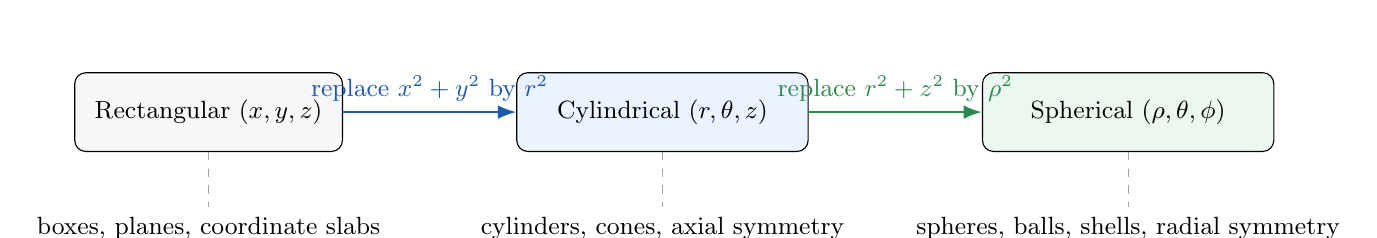
\begin{tikzpicture}[node distance=1.5cm, font=\small]
\node[draw,rounded corners,fill=softgray,minimum width=3.4cm,minimum height=1cm] (rect) {Rectangular $(x,y,z)$};
\node[draw,rounded corners,fill=softblue,right=2.2cm of rect,minimum width=3.7cm,minimum height=1cm] (cyl) {Cylindrical $(r,\theta,z)$};
\node[draw,rounded corners,fill=softgreen,right=2.2cm of cyl,minimum width=3.7cm,minimum height=1cm] (sph) {Spherical $(\rho,\theta,\phi)$};
\node[below=0.7cm of rect,align=center] (rtext) {boxes, planes,\ coordinate slabs};
\node[below=0.7cm of cyl,align=center] (ctext) {cylinders, cones,\ axial symmetry};
\node[below=0.7cm of sph,align=center] (stext) {spheres, balls,\ shells, radial symmetry};
\draw[-Latex,thick,chapterblue] (rect) -- node[above]{replace $x^2+y^2$ by $r^2$} (cyl);
\draw[-Latex,thick,chaptergreen] (cyl) -- node[above]{replace $r^2+z^2$ by $\rho^2$} (sph);
\draw[guide] (rect) -- (rtext);
\draw[guide] (cyl) -- (ctext);
\draw[guide] (sph) -- (stext);
\end{tikzpicture}
\caption{Coordinate systems as languages for geometry. The best language is usually the one whose coordinate surfaces match the boundary surfaces.}
\end{figure}

\section{Learning goals}

After studying this chapter, you should be able to:
\begin{enumerate}
  \item convert points and equations among rectangular, cylindrical, and spherical coordinates;
  \item recognize common coordinate surfaces: cylinders, cones, spheres, and half-planes;
  \item use the volume elements $dV=r\,dz\,dr\,d\theta$ and $dV=\rho^2\sin\phi\,d\rho\,d\phi\,d\theta$;
  \item set up and evaluate triple integrals in cylindrical coordinates;
  \item set up and evaluate triple integrals in spherical coordinates;
  \item choose an efficient coordinate system by reading the symmetry of the region and integrand;
  \item use coordinate transformations in probability, statistics, and simulation.
\end{enumerate}

\section{Why new coordinates are needed}

A coordinate system is a language for describing points. Rectangular coordinates describe a point by three signed distances $(x,y,z)$. This is perfect for a rectangular box such as
\[
0\le x\le 2,\qquad 1\le y\le 4,\qquad -1\le z\le 3.
\]
But the cylinder $x^2+y^2\le 4$ and the sphere $x^2+y^2+z^2\le 9$ already contain distance expressions. That is the signal that radial coordinates may simplify the problem.

\begin{workflowbox}[Coordinate choice principle]
Use a coordinate system whose coordinate surfaces resemble the boundary surfaces of the region.
\begin{itemize}
  \item Cylinders suggest cylindrical coordinates.
  \item Spheres suggest spherical coordinates.
  \item Cones often work well in either cylindrical or spherical coordinates.
  \item Planes and boxes often work well in rectangular coordinates.
\end{itemize}
\end{workflowbox}

\section{Cylindrical coordinates}

\begin{definitionbox}[Cylindrical coordinates]
Cylindrical coordinates combine polar coordinates in the $xy$-plane with the usual vertical coordinate $z$:
\[
x=r\cos\theta,\qquad y=r\sin\theta,\qquad z=z.
\]
Here $r\ge 0$ and usually $0\le \theta\le 2\pi$. The inverse relations are
\[
r^2=x^2+y^2,\qquad \tan\theta=\frac{y}{x},\qquad z=z.
\]
The number $r$ is the distance from $(x,y,z)$ to the $z$-axis, not the distance to the origin in space.
\end{definitionbox}

\begin{center}
\begin{tabular}{lll}
\toprule
Cylindrical equation & Geometric meaning & Rectangular form \\
\midrule
$r=r_0$ & cylinder around the $z$-axis & $x^2+y^2=r_0^2$ \\
$\theta=\theta_0$ & vertical half-plane & $y=(\tan\theta_0)x$ with orientation \\
$z=z_0$ & horizontal plane & $z=z_0$ \\
$z=cr$ & cone & $z=c\sqrt{x^2+y^2}$ \\
\bottomrule
\end{tabular}
\end{center}

\begin{figure}[H]
\centering
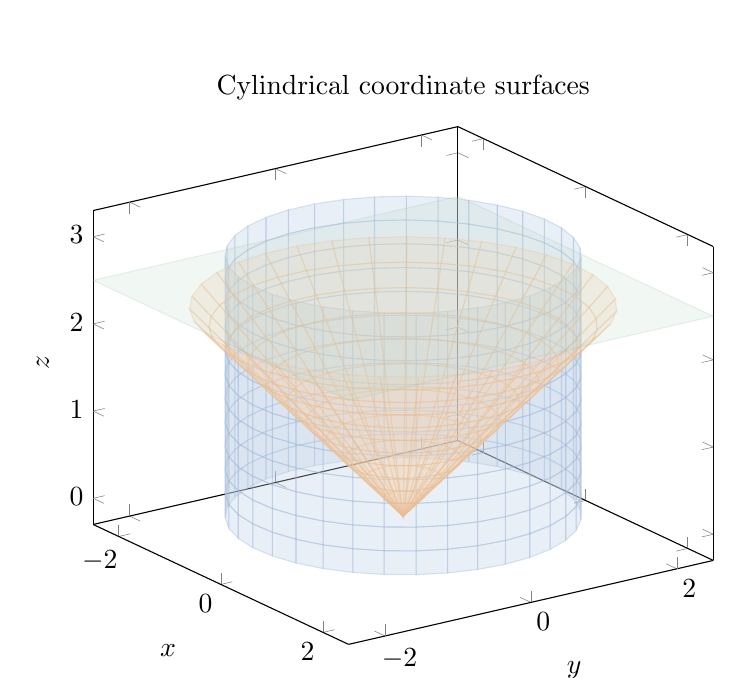
\begin{tikzpicture}
\begin{axis}[
  width=0.78\textwidth,
  view={55}{25},
  xlabel={$x$},ylabel={$y$},zlabel={$z$},
  domain=0:360,y domain=0:3,
  samples=36,samples y=12,
  z buffer=sort,
  title={Cylindrical coordinate surfaces}
]
\addplot3[surf,shader=flat,draw=chapterblue!45,fill=chapterblue!28,opacity=.35] ({2*cos(x)},{2*sin(x)},{y});
\addplot3[surf,shader=flat,draw=chapterorange!55,fill=chapterorange!35,opacity=.32,domain=0:360,y domain=0:2.4,samples=36,samples y=12] ({y*cos(x)},{y*sin(x)},{y});
\addplot3[surf,shader=flat,draw=chaptergreen!50,fill=chaptergreen!30,opacity=.22,domain=-2.5:2.5,y domain=-2.5:2.5,samples=2,samples y=2] ({x},{y},{2.5});
\end{axis}
\end{tikzpicture}
\caption{Basic cylindrical coordinate surfaces: a cylinder $r=2$, a cone $z=r$, and a horizontal plane $z=2.5$.}
\end{figure}

\section{The cylindrical volume element}

In rectangular coordinates, a small box has volume $dV=dx\,dy\,dz$. In cylindrical coordinates, a small coordinate box has dimensions approximately
\[
dr,\qquad r\,d\theta,\qquad dz.
\]
Therefore
\[
dV=r\,dz\,dr\,d\theta.
\]
The factor $r$ accounts for the fact that an angular change $d\theta$ sweeps out a longer arc when $r$ is larger.

\begin{figure}[H]
\centering
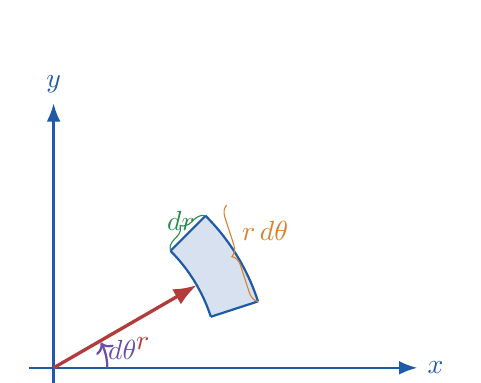
\begin{tikzpicture}[scale=1.05]
  \draw[axisline] (-0.3,0) -- (4.4,0) node[right] {$x$};
  \draw[axisline] (0,-0.3) -- (0,3.2) node[above] {$y$};
  \def\rA{2.0}
  \def\rB{2.6}
  \def\aA{18}
  \def\aB{45}
  \fill[chapterblue!18] (\aA:\rA) arc (\aA:\aB:\rA) -- (\aB:\rB) arc (\aB:\aA:\rB) -- cycle;
  \draw[chapterblue,thick] (\aA:\rA) arc (\aA:\aB:\rA);
  \draw[chapterblue,thick] (\aA:\rB) arc (\aA:\aB:\rB);
  \draw[chapterblue,thick] (\aA:\rA) -- (\aA:\rB);
  \draw[chapterblue,thick] (\aB:\rA) -- (\aB:\rB);
  \draw[vector] (0,0) -- (30:\rA) node[midway,below right] {$r$};
  \draw[decorate,decoration={brace,amplitude=4pt},chapterorange] (\aA:\rB) arc (\aA:\aB:\rB);
  \node[chapterorange] at (33:3.05) {$r\,d\theta$};
  \draw[decorate,decoration={brace,amplitude=4pt},chaptergreen] (\aB:\rA) -- (\aB:\rB);
  \node[chaptergreen] at (49:2.35) {$dr$};
  \draw[->,chapterpurple,thick] (0.65,0) arc (0:28:0.65);
  \node[chapterpurple] at (0.83,0.22) {$d\theta$};
\end{tikzpicture}
\caption{The polar base of a cylindrical volume element. Multiplying the base dimensions $dr$ and $r\,d\theta$ by height $dz$ gives $dV=r\,dz\,dr\,d\theta$.}
\end{figure}

\begin{mainideabox}[Cylindrical integration formula]
If $x=r\cos\theta$, $y=r\sin\theta$, and $z=z$, then
\[
\iiintE f(x,y,z)\,dV
=\int_{\theta=\alpha}^{\beta}\int_{r=h_1(\theta)}^{h_2(\theta)}
\int_{z=g_1(r,\theta)}^{g_2(r,\theta)}
f(r\cos\theta,r\sin\theta,z)\,r\,dz\,dr\,d\theta.
\]
The extra factor $r$ is not optional. It is part of the volume element.
\end{mainideabox}

\section{Worked examples in cylindrical coordinates}

\begin{examplebox}[Example 1: Convert a point]
Find rectangular coordinates for $(r,\theta,z)=\left(2,\frac{2\pi}{3},3\right)$. Using $x=r\cos\theta$ and $y=r\sin\theta$,
\[
x=2\cos\left(\frac{2\pi}{3}\right)=-1,
\qquad
y=2\sin\left(\frac{2\pi}{3}\right)=\sqrt3,
\]
and $z=3$. Thus the rectangular coordinates are $(-1,\sqrt3,3)$.
\end{examplebox}

\begin{examplebox}[Example 2: A cone below a plane]
Find the volume of the solid above the cone $z=r$ and below the plane $z=1$.
The cone and plane intersect when $r=1$. The region is
\[
0\le \theta\le 2\pi,\qquad 0\le r\le 1,\qquad r\le z\le 1.
\]
Thus
\[
V=\int_0^{2\pi}\int_0^1\int_r^1 r\,dz\,dr\,d\theta
=2\pi\int_0^1 r(1-r)\,dr=\frac{\pi}{3}.
\]
\end{examplebox}

\begin{figure}[H]
\centering
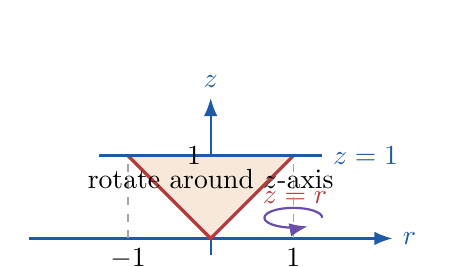
\begin{tikzpicture}[scale=1.05]
\draw[axisline] (-2.2,0) -- (2.2,0) node[right] {$r$};
\draw[axisline] (0,-0.2) -- (0,1.7) node[above] {$z$};
\fill[chapterorange!18] (-1,1) -- (0,0) -- (1,1) -- cycle;
\draw[chapterred,very thick] (-1,1) -- (0,0) -- (1,1) node[midway,right] {$z=r$};
\draw[chapterblue,very thick] (-1.35,1) -- (1.35,1) node[right] {$z=1$};
\draw[guide] (1,0) -- (1,1);
\draw[guide] (-1,0) -- (-1,1);
\node[below] at (1,0) {$1$};
\node[below] at (-1,0) {$-1$};
\node[left] at (0,1) {$1$};
\node at (0,0.72) {rotate around $z$-axis};
\draw[-Latex,chapterpurple,thick] (1.35,0.25) arc[start angle=0,end angle=300,x radius=0.35,y radius=0.12];
\end{tikzpicture}
\caption{A cross-section of the solid above $z=r$ and below $z=1$. Cylindrical coordinates turn the solid into $0\le r\le 1$, $r\le z\le 1$.}
\end{figure}

\begin{examplebox}[Example 3: A cylinder above a paraboloid]
Let $E$ be the solid inside $x^2+y^2\le 1$, above the paraboloid $z=1-x^2-y^2$, and below the plane $z=3$. Since $x^2+y^2=r^2$, the bounds are
\[
0\le \theta\le 2\pi,\qquad 0\le r\le 1,\qquad 1-r^2\le z\le 3.
\]
Hence
\[
V=\int_0^{2\pi}\int_0^1\int_{1-r^2}^{3} r\,dz\,dr\,d\theta
=2\pi\int_0^1 r(2+r^2)\,dr=\frac{5\pi}{2}.
\]
\end{examplebox}

\begin{figure}[H]
\centering
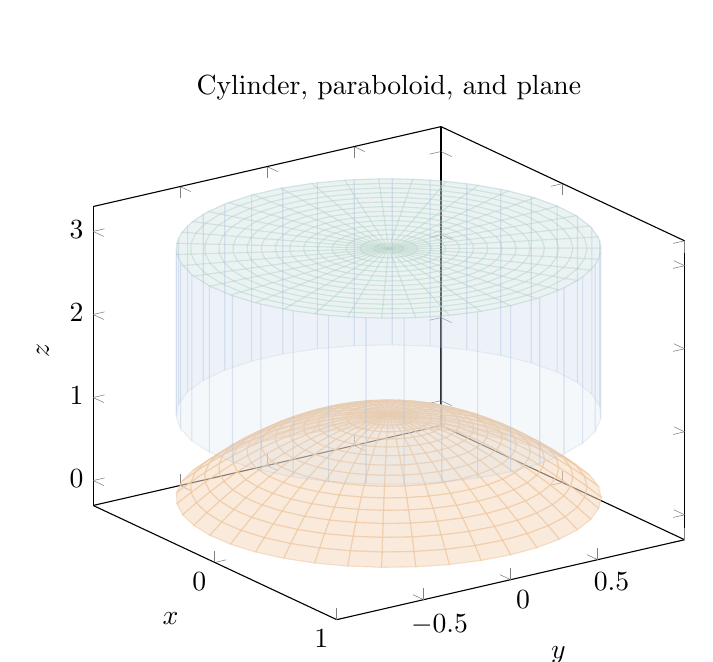
\begin{tikzpicture}
\begin{axis}[
  width=0.75\textwidth,
  view={55}{25},
  xlabel={$x$},ylabel={$y$},zlabel={$z$},
  domain=0:360,y domain=0:1,
  samples=40,samples y=16,
  z buffer=sort,
  title={Cylinder, paraboloid, and plane}
]
\addplot3[surf,shader=flat,draw=chapterorange!45,fill=chapterorange!30,opacity=.55] ({y*cos(x)},{y*sin(x)},{1-y^2});
\addplot3[surf,shader=flat,draw=chaptergreen!40,fill=chaptergreen!20,opacity=.30] ({y*cos(x)},{y*sin(x)},{3});
\addplot3[surf,shader=flat,draw=chapterblue!40,fill=chapterblue!20,opacity=.22,domain=0:360,y domain=1:3,samples=36,samples y=2] ({cos(x)},{sin(x)},{y});
\end{axis}
\end{tikzpicture}
\caption{A solid inside the cylinder $r=1$, above $z=1-r^2$, and below $z=3$.}
\end{figure}

\begin{examplebox}[Example 4: Mass with radial density]
For the same solid $E$, suppose $\delta(x,y,z)=\sqrt{x^2+y^2}$. In cylindrical coordinates, $\delta=r$. Mass is density integrated over volume:
\[
M=\int_0^{2\pi}\int_0^1\int_{1-r^2}^{3} r\cdot r\,dz\,dr\,d\theta.
\]
The first $r$ is the density and the second $r$ is the Jacobian factor. Therefore
\[
M=2\pi\int_0^1 r^2(2+r^2)\,dr
=2\pi\left(\frac{2}{3}+\frac15\right)=\frac{26\pi}{15}.
\]
\end{examplebox}

\begin{examplebox}[Example 5: Converting a rectangular integral]
Evaluate
\[
\int_{-1}^{1}\int_{-\sqrt{1-x^2}}^{\sqrt{1-x^2}}\int_{\sqrt{x^2+y^2}}^{1} (x^2+y^2)\,dz\,dy\,dx.
\]
The projection onto the $xy$-plane is the unit disk. The lower surface is the cone $z=\sqrt{x^2+y^2}=r$, the upper surface is $z=1$, and the integrand becomes $r^2$. Therefore
\[
\int_0^{2\pi}\int_0^1\int_r^1 r^2\,r\,dz\,dr\,d\theta
=2\pi\int_0^1 r^3(1-r)\,dr=\frac{\pi}{10}.
\]
\end{examplebox}

\section{Spherical coordinates}

\begin{definitionbox}[Spherical coordinates]
Spherical coordinates describe a point by $(\rho,\theta,\phi)$, where $\rho$ is the distance from the origin, $\theta$ is the angle in the $xy$-plane measured from the positive $x$-axis, and $\phi$ is the angle from the positive $z$-axis. The conversion formulas are
\[
x=\rho\sin\phi\cos\theta,
\qquad
y=\rho\sin\phi\sin\theta,
\qquad
z=\rho\cos\phi.
\]
Usually $\rho\ge 0$, $0\le \theta\le 2\pi$, and $0\le \phi\le \pi$. The relations with cylindrical coordinates are
\[
r=\rho\sin\phi,\qquad z=\rho\cos\phi,\qquad \theta=\theta.
\]
\end{definitionbox}

\begin{figure}[H]
\centering
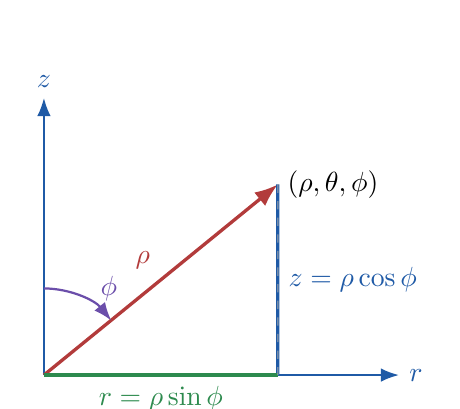
\begin{tikzpicture}[scale=1.1]
\draw[axisline] (0,0) -- (4.1,0) node[right] {$r$};
\draw[axisline] (0,0) -- (0,3.2) node[above] {$z$};
\coordinate (O) at (0,0);
\coordinate (P) at (2.7,2.2);
\draw[vector] (O) -- (P) node[midway,above left] {$\rho$};
\draw[chapterblue,very thick] (P) -- (2.7,0) node[midway,right] {$z=\rho\cos\phi$};
\draw[chaptergreen,very thick] (O) -- (2.7,0) node[midway,below] {$r=\rho\sin\phi$};
\draw[chapterpurple,thick,-Latex] (0,1.0) arc[start angle=90,end angle=39, radius=1.0];
\node[chapterpurple] at (0.75,1.0) {$\phi$};
\fill[point] (P) circle;
\node[right] at (P) {$(\rho,\theta,\phi)$};
\draw[guide] (P) -- (2.7,0);
\end{tikzpicture}
\caption{In a vertical cross-section through the $z$-axis, spherical coordinates reduce to right-triangle geometry: $r=\rho\sin\phi$ and $z=\rho\cos\phi$.}
\end{figure}

\begin{center}
\begin{tabular}{lll}
\toprule
Spherical equation & Geometric meaning & Rectangular or cylindrical form \\
\midrule
$\rho=\rho_0$ & sphere centered at origin & $x^2+y^2+z^2=\rho_0^2$ \\
$\theta=\theta_0$ & vertical half-plane & same as cylindrical angle \\
$\phi=\phi_0$ & cone with vertex at origin & $z=r\cot\phi_0$ \\
\bottomrule
\end{tabular}
\end{center}

\begin{figure}[H]
\centering
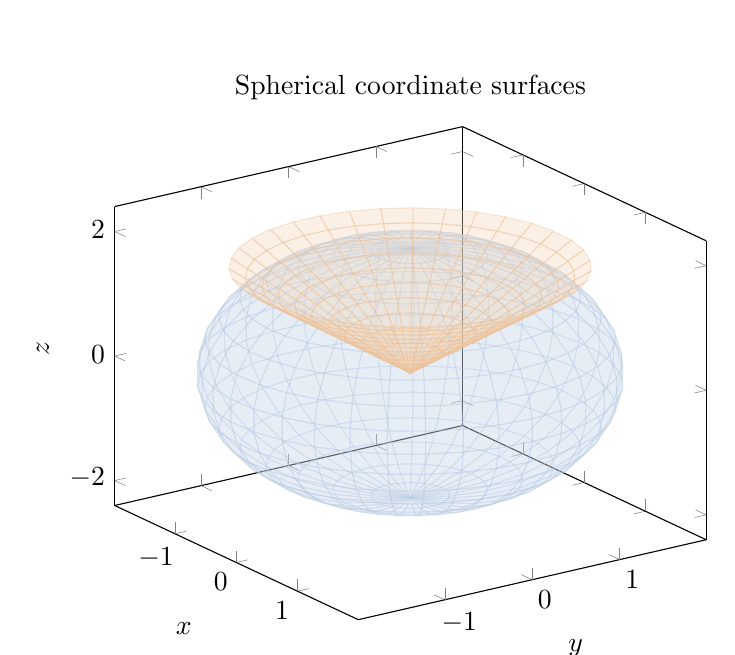
\begin{tikzpicture}
\begin{axis}[
  width=0.75\textwidth,
  view={55}{25},
  xlabel={$x$},ylabel={$y$},zlabel={$z$},
  domain=0:360,y domain=0:180,
  samples=36,samples y=18,
  z buffer=sort,
  title={Spherical coordinate surfaces}
]
\addplot3[surf,shader=flat,draw=chapterblue!35,fill=chapterblue!25,opacity=.25] ({2*sin(y)*cos(x)},{2*sin(y)*sin(x)},{2*cos(y)});
\addplot3[surf,shader=flat,draw=chapterorange!50,fill=chapterorange!35,opacity=.35,domain=0:360,y domain=0:2.4,samples=36,samples y=12] ({y*sin(45)*cos(x)},{y*sin(45)*sin(x)},{y*cos(45)});
\end{axis}
\end{tikzpicture}
\caption{Basic spherical coordinate surfaces: the sphere $\rho=2$ and the cone $\phi=\pi/4$.}
\end{figure}

\section{The spherical volume element}

A small spherical coordinate box has approximate side lengths
\[
d\rho,\qquad \rho\,d\phi,\qquad \rho\sin\phi\,d\theta.
\]
Therefore
\[
dV=\rho^2\sin\phi\,d\rho\,d\phi\,d\theta.
\]

\begin{figure}[H]
\centering
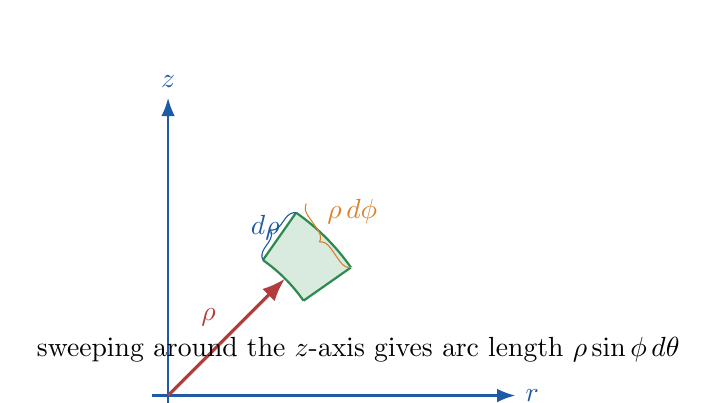
\begin{tikzpicture}[scale=1.05]
\draw[axisline] (-0.2,0) -- (4.2,0) node[right] {$r$};
\draw[axisline] (0,-0.2) -- (0,3.6) node[above] {$z$};
\def\ra{2.0}
\def\rb{2.7}
\def\phia{35}
\def\phib{55}
\fill[chaptergreen!18] (\phia:\ra) arc(\phia:\phib:\ra) -- (\phib:\rb) arc(\phib:\phia:\rb) -- cycle;
\draw[chaptergreen,thick] (\phia:\ra) arc(\phia:\phib:\ra);
\draw[chaptergreen,thick] (\phia:\rb) arc(\phia:\phib:\rb);
\draw[chaptergreen,thick] (\phia:\ra) -- (\phia:\rb);
\draw[chaptergreen,thick] (\phib:\ra) -- (\phib:\rb);
\draw[vector] (0,0) -- (45:\ra) node[midway,above left] {$\rho$};
\draw[decorate,decoration={brace,amplitude=4pt},chapterorange] (\phia:\rb) arc(\phia:\phib:\rb);
\node[chapterorange] at (45:3.15) {$\rho\,d\phi$};
\draw[decorate,decoration={brace,amplitude=4pt},chapterblue] (\phib:\ra) -- (\phib:\rb);
\node[chapterblue] at (60:2.35) {$d\rho$};
\node[align=center] at (2.3,0.55) {sweeping around the $z$-axis\ gives arc length $\rho\sin\phi\,d\theta$};
\end{tikzpicture}
\caption{The spherical volume factor is a product of three local lengths: $d\rho$, $\rho\,d\phi$, and $\rho\sin\phi\,d\theta$.}
\end{figure}

\begin{mainideabox}[Spherical integration formula]
If
\[
x=\rho\sin\phi\cos\theta,\qquad y=\rho\sin\phi\sin\theta,\qquad z=\rho\cos\phi,
\]
then
\[
\iiintE f(x,y,z)\,dV
=\int\!\int\!\int f(\rho\sin\phi\cos\theta,\rho\sin\phi\sin\theta,\rho\cos\phi)
\rho^2\sin\phi\,d\rho\,d\phi\,d\theta.
\]
The factor $\rho^2\sin\phi$ is the three-dimensional Jacobian factor for spherical coordinates.
\end{mainideabox}

\section{Worked examples in spherical coordinates}

\begin{examplebox}[Example 6: Volume of the unit ball]
For the unit ball $x^2+y^2+z^2\le 1$, spherical bounds are
\[
0\le \rho\le 1,\qquad 0\le \phi\le \pi,\qquad 0\le \theta\le 2\pi.
\]
Thus
\[
V=\int_0^{2\pi}\int_0^\pi\int_0^1 \rho^2\sin\phi\,d\rho\,d\phi\,d\theta
=(2\pi)(2)\left(\frac13\right)=\frac{4\pi}{3}.
\]
\end{examplebox}

\begin{examplebox}[Example 7: Inside a sphere and above a cone]
Find the volume inside $x^2+y^2+z^2=8$ and above $z=\sqrt{x^2+y^2}$. The sphere is $\rho=\sqrt8$. The cone is $z=r$, so
\[
\rho\cos\phi=\rho\sin\phi,
\]
which gives $\phi=\pi/4$ away from the origin. Hence
\[
0\le \theta\le 2\pi,
\qquad 0\le \phi\le \frac{\pi}{4},
\qquad 0\le \rho\le \sqrt8.
\]
Therefore
\[
V=\int_0^{2\pi}\int_0^{\pi/4}\int_0^{\sqrt8}\rho^2\sin\phi\,d\rho\,d\phi\,d\theta
=\frac{32\pi}{3}(\sqrt2-1).
\]
\end{examplebox}

\begin{figure}[H]
\centering
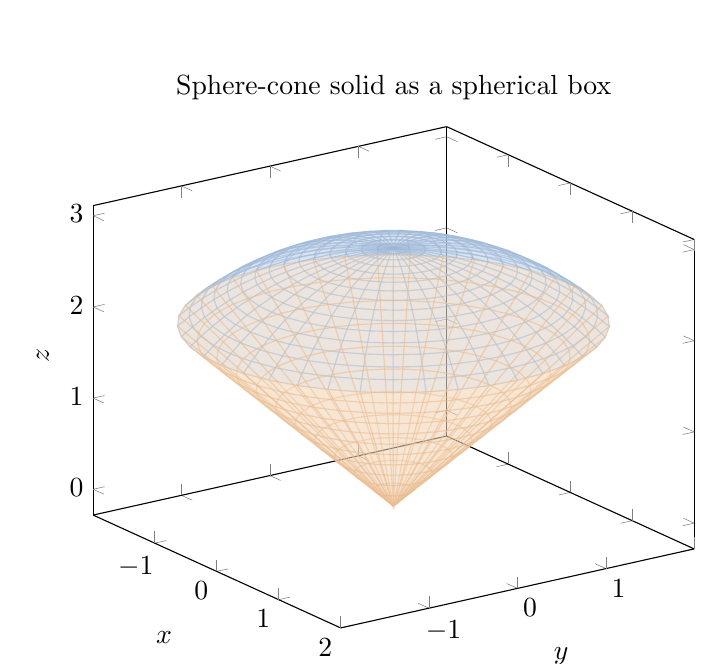
\begin{tikzpicture}
\begin{axis}[
  width=0.76\textwidth,
  view={55}{24},
  xlabel={$x$},ylabel={$y$},zlabel={$z$},
  domain=0:360,y domain=0:45,
  samples=42,samples y=16,
  z buffer=sort,
  title={Sphere-cone solid as a spherical box}
]
\addplot3[surf,shader=flat,draw=chapterblue!45,fill=chapterblue!25,opacity=.42] ({2.828*sin(y)*cos(x)},{2.828*sin(y)*sin(x)},{2.828*cos(y)});
\addplot3[surf,shader=flat,draw=chapterorange!55,fill=chapterorange!35,opacity=.35,domain=0:360,y domain=0:2.828,samples=42,samples y=12] ({y*sin(45)*cos(x)},{y*sin(45)*sin(x)},{y*cos(45)});
\end{axis}
\end{tikzpicture}
\caption{The region inside a sphere and above a cone becomes a simple rectangular box in $(\rho,\phi,\theta)$-space.}
\end{figure}

\begin{examplebox}[Example 8: A spherical shell in the first octant]
Let $E$ be the part of the spherical shell $1\le x^2+y^2+z^2\le 4$ in the first octant. The first octant means $x,y,z\ge 0$, so
\[
0\le \theta\le \frac{\pi}{2},\qquad 0\le \phi\le \frac{\pi}{2}.
\]
The shell condition gives $1\le \rho\le 2$. Hence
\[
V=\int_0^{\pi/2}\int_0^{\pi/2}\int_1^2 \rho^2\sin\phi\,d\rho\,d\phi\,d\theta
=\left(\frac{\pi}{2}\right)(1)\left(\frac{2^3-1^3}{3}\right)=\frac{7\pi}{6}.
\]
\end{examplebox}

\begin{figure}[H]
\centering
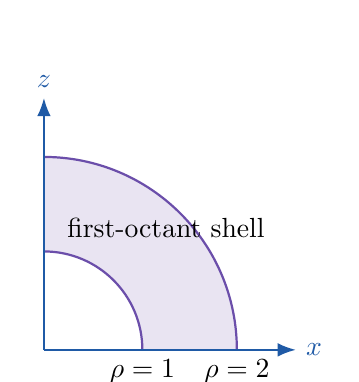
\begin{tikzpicture}[scale=1.0]
\draw[axisline] (0,0) -- (3.2,0) node[right] {$x$};
\draw[axisline] (0,0) -- (0,3.2) node[above] {$z$};
\fill[chapterpurple!15] (0:1.25) arc(0:90:1.25) -- (90:2.45) arc(90:0:2.45) -- cycle;
\draw[chapterpurple,thick] (0:1.25) arc(0:90:1.25);
\draw[chapterpurple,thick] (0:2.45) arc(0:90:2.45);
\draw[chapterblue,thick] (0,0) -- (3,0);
\draw[chapterblue,thick] (0,0) -- (0,3);
\node at (1.55,1.55) {first-octant shell};
\node[below] at (1.25,0) {$\rho=1$};
\node[below] at (2.45,0) {$\rho=2$};
\end{tikzpicture}
\caption{A cross-section of the first-octant spherical shell. The full three-dimensional region has $0\le\theta\le\pi/2$ and $0\le\phi\le\pi/2$.}
\end{figure}

\section{Choosing among rectangular, cylindrical, and spherical coordinates}

Coordinate choice is part of problem solving. A good choice makes the region and integrand simple. A poor choice may make a straightforward problem unnecessarily complicated.

\begin{center}
\begin{tabularx}{\textwidth}{>{\raggedright\arraybackslash}p{0.34\textwidth}>{\raggedright\arraybackslash}p{0.22\textwidth}>{\raggedright\arraybackslash}X}
\toprule
Geometry or expression & Recommended coordinates & Reason \\
\midrule
Box with constant $x,y,z$ bounds & rectangular & boundaries already align with coordinate planes \\
Cylinder $x^2+y^2=R^2$ & cylindrical & becomes $r=R$ \\
Cone $z=c\sqrt{x^2+y^2}$ & cylindrical or spherical & becomes $z=cr$ or $\phi=$ constant \\
Sphere $x^2+y^2+z^2=R^2$ & spherical & becomes $\rho=R$ \\
Radial integrand $f(x^2+y^2)$ & cylindrical & becomes $f(r^2)$ \\
Radial integrand $f(x^2+y^2+z^2)$ & spherical & becomes $f(\rho^2)$ \\
First octant of a ball & spherical & constant angle bounds \\
Solid of revolution around the $z$-axis & cylindrical & natural $r$ and $z$ description \\
\bottomrule
\end{tabularx}
\end{center}

\begin{workflowbox}[A practical workflow]
\begin{enumerate}
  \item Sketch or identify the boundary surfaces.
  \item Translate the boundary equations into candidate coordinate systems.
  \item Choose the system where most bounds become constants or simple functions.
  \item Rewrite the integrand.
  \item Include the correct volume element.
\end{enumerate}
\end{workflowbox}

\section{Numerical integration in cylindrical and spherical coordinates}

The coordinate formulas are useful not only for exact integration but also for computation. A numerical method works best when the region has simple bounds. For the sphere-cone solid from Example 7,
\[
0\le \theta\le 2\pi,\qquad 0\le \phi\le \frac{\pi}{4},\qquad 0\le \rho\le \sqrt8.
\]
A grid-based spherical-coordinate sum approximates the volume by
\[
\sum \rho_{ijk}^2\sin\phi_j\,\Delta\rho\,\Delta\phi\,\Delta\theta.
\]

\begin{figure}[H]
\centering
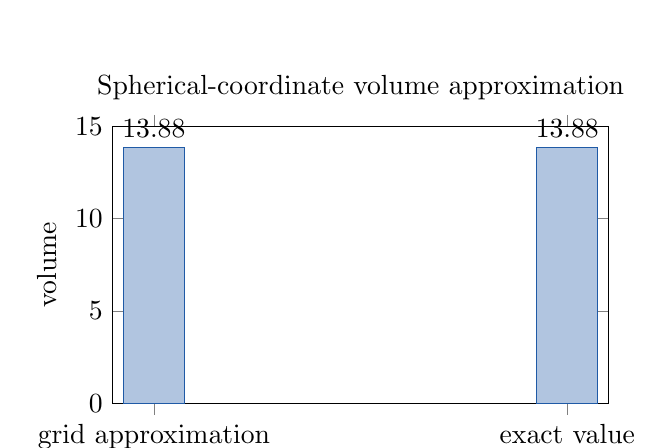
\begin{tikzpicture}
\begin{axis}[
  ybar,
  width=0.65\textwidth,
  height=0.42\textwidth,
  ymin=0,ymax=15,
  ylabel={volume},
  symbolic x coords={grid approximation,exact value},
  xtick=data,
  nodes near coords,
  nodes near coords align={vertical},
  bar width=22pt,
  title={Spherical-coordinate volume approximation}
]
\addplot[fill=chapterblue!35,draw=chapterblue] coordinates {(grid approximation,13.88) (exact value,13.88)};
\end{axis}
\end{tikzpicture}
\caption{For regions with spherical bounds, a grid in $(\rho,\phi,\theta)$ directly matches the geometry.}
\end{figure}

\section{Coordinate transformations and probability}

Triple integrals are also probability integrals. If $f(x,y,z)$ is a joint density, then
\[
P((X,Y,Z)\in E)=\iiint_E f(x,y,z)\,dV.
\]
When the density is radially symmetric, spherical coordinates are natural. For example, the three-dimensional standard normal density is
\[
f(x,y,z)=\frac{1}{(2\pi)^{3/2}}e^{-(x^2+y^2+z^2)/2}.
\]
Since $x^2+y^2+z^2=\rho^2$, spherical coordinates give
\[
f=\frac{1}{(2\pi)^{3/2}}e^{-\rho^2/2}.
\]
The probability mass in a ball of radius $R$ is
\[
P(\rho\le R)=\int_0^{2\pi}\int_0^\pi\int_0^R
\frac{1}{(2\pi)^{3/2}}e^{-\rho^2/2}\rho^2\sin\phi\,d\rho\,d\phi\,d\theta.
\]
After integrating out the angles,
\[
P(\rho\le R)=\sqrt{\frac{2}{\pi}}\int_0^R \rho^2e^{-\rho^2/2}\,d\rho.
\]

\begin{figure}[H]
\centering
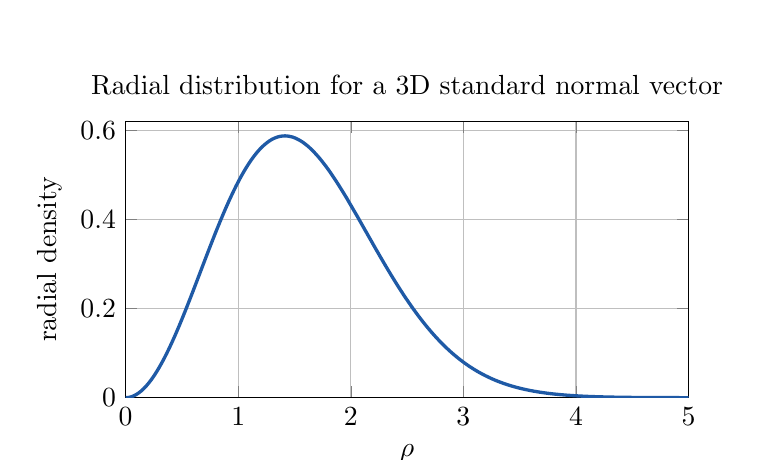
\begin{tikzpicture}
\begin{axis}[
  width=0.72\textwidth,
  height=0.42\textwidth,
  xmin=0,xmax=5,
  ymin=0,ymax=0.62,
  xlabel={$\rho$},ylabel={radial density},
  grid=both,
  title={Radial distribution for a 3D standard normal vector}
]
\addplot[very thick,chapterblue,domain=0:5,samples=220] {sqrt(2/pi)*x^2*exp(-x^2/2)};
\end{axis}
\end{tikzpicture}
\caption{A rotationally symmetric three-dimensional density becomes a one-dimensional radial density after integrating out angular variables.}
\end{figure}

\section{Sampling uniformly from a ball}

Coordinate transformations matter in simulation. To sample uniformly from the unit ball in $\R^3$, it is not correct to choose $\rho$ uniformly from $[0,1]$. The volume element contains $\rho^2$, so more volume lies near the boundary.

A correct method is
\[
\theta=2\pi U_1,\qquad \cos\phi=2U_2-1,\qquad \rho=U_3^{1/3},
\]
where $U_1,U_2,U_3$ are independent uniform random variables on $[0,1]$. The power $1/3$ appears because the volume of a ball of radius $r$ is proportional to $r^3$.

\begin{figure}[H]
\centering
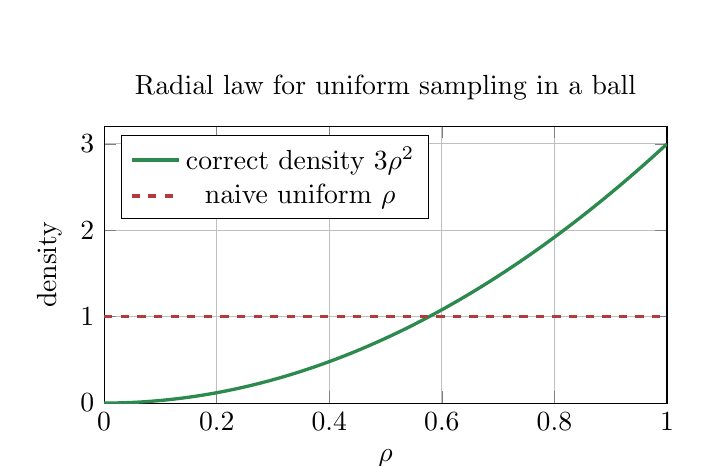
\begin{tikzpicture}
\begin{axis}[
  width=0.72\textwidth,
  height=0.42\textwidth,
  xmin=0,xmax=1,
  ymin=0,ymax=3.2,
  xlabel={$\rho$},ylabel={density},
  grid=both,
  legend style={at={(0.03,0.97)},anchor=north west,fill=white},
  title={Radial law for uniform sampling in a ball}
]
\addplot[very thick,chaptergreen,domain=0:1,samples=150] {3*x^2};
\addlegendentry{correct density $3\rho^2$}
\addplot[very thick,chapterred,dashed,domain=0:1,samples=2] {1};
\addlegendentry{naive uniform $\rho$}
\end{axis}
\end{tikzpicture}
\caption{Uniform volume sampling has radial density $3\rho^2$, not a flat radial density.}
\end{figure}

\section{Common mistakes}

\begin{warningbox}[Mistake 1: Forgetting the Jacobian factor]
In cylindrical coordinates, the volume element is $r\,dz\,dr\,d\theta$, not just $dz\,dr\,d\theta$. In spherical coordinates, the volume element is $\rho^2\sin\phi\,d\rho\,d\phi\,d\theta$, not just $d\rho\,d\phi\,d\theta$.
\end{warningbox}

\begin{warningbox}[Mistake 2: Confusing $r$ and $\rho$]
In cylindrical coordinates, $r=\sqrt{x^2+y^2}$. In spherical coordinates, $\rho=\sqrt{x^2+y^2+z^2}$. Thus $r$ is distance to the $z$-axis, while $\rho$ is distance to the origin.
\end{warningbox}

\begin{warningbox}[Mistake 3: Confusing $\theta$ and $\phi$]
The angle $\theta$ is measured in the $xy$-plane. The angle $\phi$ is measured down from the positive $z$-axis.
\end{warningbox}

\begin{warningbox}[Mistake 4: Writing bounds before understanding the geometry]
Do not begin by guessing bounds. First translate the boundary surfaces. Then decide which coordinate system makes them simple.
\end{warningbox}

\section{Chapter summary}

Cylindrical coordinates are defined by
\[
x=r\cos\theta,\qquad y=r\sin\theta,\qquad z=z,
\]
with volume element
\[
dV=r\,dz\,dr\,d\theta.
\]
Spherical coordinates are defined by
\[
x=\rho\sin\phi\cos\theta,\qquad y=\rho\sin\phi\sin\theta,\qquad z=\rho\cos\phi,
\]
with volume element
\[
dV=\rho^2\sin\phi\,d\rho\,d\phi\,d\theta.
\]
The main problem-solving skill is choosing coordinates that match the region and integrand. Cylindrical coordinates simplify cylinders, cones, and axial symmetry. Spherical coordinates simplify spheres, balls, shells, cones, and radial functions.

\section{Practice problems}

\begin{enumerate}
  \item Convert the cylindrical point $(4,\pi/6,2)$ to rectangular coordinates.
  \item Convert the rectangular point $(1,1,3)$ to cylindrical coordinates.
  \item Describe the surface $r=5$ in rectangular coordinates.
  \item Describe the surface $z=2r$ in rectangular coordinates.
  \item Find the volume inside $x^2+y^2=9$ between $z=0$ and $z=4$.
  \item Find the mass of the solid in Problem 5 if the density is $\delta(x,y,z)=x^2+y^2$.
  \item Set up a cylindrical-coordinate integral for the volume under $z=4-x^2-y^2$ and above the $xy$-plane.
  \item Evaluate the integral from Problem 7.
  \item Convert the spherical point $(\rho,\theta,\phi)=(2,\pi/3,\pi/4)$ to rectangular coordinates.
  \item Describe the surface $\rho=3$ in rectangular coordinates.
  \item Describe the surface $\phi=\pi/3$ in rectangular coordinates.
  \item Find the volume of the ball $x^2+y^2+z^2\le 27$.
  \item Find the volume of the upper hemisphere $x^2+y^2+z^2\le 9$, $z\ge 0$.
  \item Set up a spherical-coordinate integral for the volume inside $x^2+y^2+z^2=16$ and above the cone $z=\sqrt{3(x^2+y^2)}$.
  \item Evaluate the integral in Problem 14.
  \item Let $E$ be the first-octant part of the ball $x^2+y^2+z^2\le 8$. Set up and evaluate a spherical-coordinate integral for its volume.
  \item Explain why choosing $\rho$ uniformly from $[0,1]$ does not produce uniform points in the unit ball.
  \item For the density $f(x,y,z)=Ce^{-(x^2+y^2+z^2)}$, write the normalization condition for $C$ using spherical coordinates.
\end{enumerate}

\section{Python lab and interactive page}

The lab for this chapter asks you to plot cylindrical and spherical coordinate surfaces, compare descriptions of the same solid, approximate triple integrals with coordinate grids, simulate points uniformly in a ball, and compare radial distributions.

\begin{itemize}
  \item Python lab: \texttt{../labs/chapter-17-cylindrical-and-spherical-coordinates.ipynb}
  \item Interactive page: \texttt{../htmls/chapter-17-cylindrical-and-spherical-coordinates.html}
\end{itemize}

\end{document}
